\documentclass{standalone}
%
\usepackage{tikz,xcolor}
\usetikzlibrary{shapes.geometric,arrows,positioning,fit}

\begin{document}
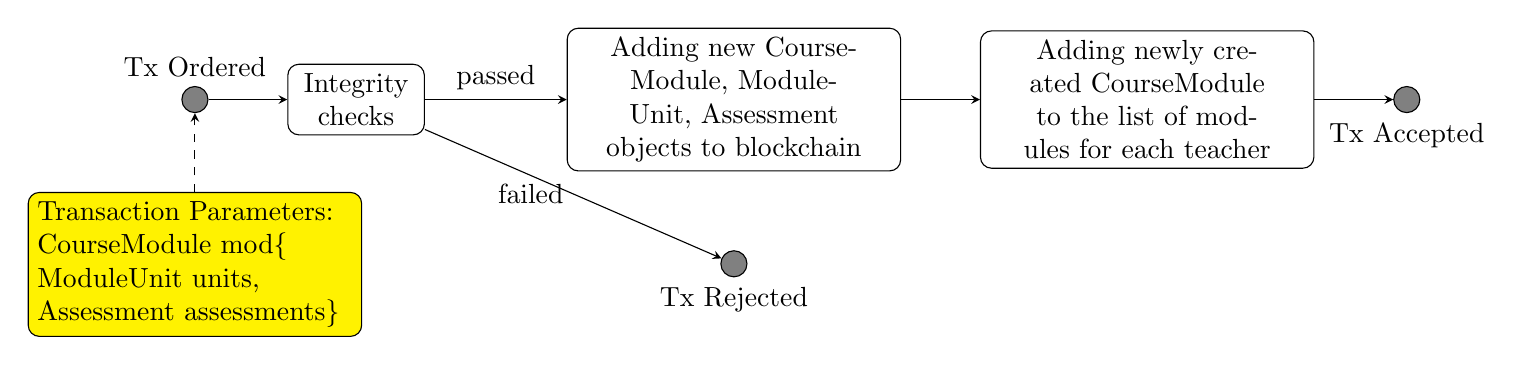
\begin{tikzpicture}[>=stealth,every node/.style={shape=rectangle,draw,rounded corners},]
    % create the nodes
    \node (start)[shape=circle, fill=gray, label=above:Tx Ordered] {};
    \node (param)[below =of start, text width=4cm, fill=yellow]{Transaction Parameters:\\CourseModule mod\{\\ModuleUnit units,\\Assessment assessments\}};   
    \node (c1) [right =of start, text width=1.5cm, align=center]{Integrity checks};
    \node (c2) [right = and 1.8cm of c1, text width=4cm, align=center]{Adding new CourseModule, ModuleUnit, Assessment objects to blockchain};
    \node (c3) [right =of c2, text width=4cm, align=center]{Adding newly created CourseModule to the list of modules for each teacher};
    \node (stop1)[below =of c2, shape=circle, fill=gray, label=below:Tx Rejected] {};        
    \node (stop2)[right = of c3, shape=circle, fill=gray, label=below:Tx Accepted] {};    
    % connect the nodes
    \draw[->, dashed] (param) to (start);        
    \draw[->] (start) to (c1);
    \draw[->] (c1) -- node[draw=none, anchor=south] {passed} (c2);
    \draw[->] (c1) -- node[draw=none, anchor=east] {failed} (stop1);    
    \draw[->] (c2) to (c3);
    \draw[->] (c3) to (stop2);    
\end{tikzpicture}
\end{document}
